\documentclass[sigconf,nonacm]{acmart}
\settopmatter{printacmref=false,printfolios=true}
\setcopyright{none}
\renewcommand\footnotetextcopyrightpermission[1]{}
\usepackage{amsmath,tabularx,array,enumitem,balance,xurl}
\setlength{\emergencystretch}{2em}
\definecolor{CourseBlue}{HTML}{315EFB}
\definecolor{CourseTeal}{HTML}{14877D}
\hypersetup{colorlinks=true,linkcolor=CourseBlue,citecolor=CourseTeal,urlcolor=CourseTeal}
\newcolumntype{Y}{>{\raggedright\arraybackslash}X}
\setlist{leftmargin=*,topsep=3pt,itemsep=2pt}
\newcommand{\CourseNumber}{COMSCI/ECON 206}
\newcommand{\CourseName}{Computational Microeconomics}
\newcommand{\CourseSession}{Autumn 2026 Session 1}
\newcommand{\Instructor}{Luyao Zhang}
\newcommand{\WorkshopSession}{Session D: Strategic AI: Trust, Collusion, and Adaptation in Repeated Interactions}

\newcommand{\GitHubLink}{\href{https://github.com/AaronW-77/ps1-overleaf-Aaron}{GitHub Repository}}
\newcommand{\ColabLink}{\href{https://colab.research.google.com/drive/1R6YTTeYsrbVoWV9td9uGGRFwsqSx7jsE?usp=sharing}{Google Colab Notebook}}
\newcommand{\DemoLink}{\href{https://huggingface.co/spaces/dku-comsci-econ206-2026/Aaron-game}{Hugging Face Game}}
\newcommand{\TemplateRepository}{\url{https://github.com/sunshineluyao/ps1-overleaf-template}}
\newcommand{\CommitHash}{PENDING}

\newcommand{\coursemeta}{\noindent\textbf{Submission to:} \CourseNumber{} --- \CourseName.\\
\textbf{Course session:} \CourseSession. \textbf{Workshop:} \WorkshopSession.\\
\textbf{Instructor:} \Instructor. \textbf{Assignment:} PS1 research proposal.\par\smallskip}
\title[AI Ticket Advice: Scarcity and Reliance]{When Should Consumers Follow AI Ticket Advice?\\Scarcity, Reliability, and Appropriate Reliance}
\author{Qianshuo (Aaron) Wang}
\affiliation{\institution{Duke Kunshan University}\city{Kunshan}\country{China}}
\email{qw124@duke.edu}
\renewcommand{\shortauthors}{Qianshuo (Aaron) Wang}

\begin{document}
\begin{teaserfigure}
\captionsetup{skip=8pt}
\centering
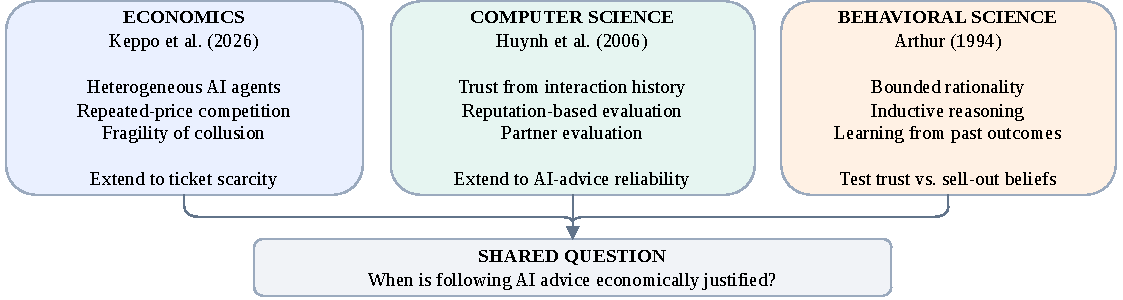
\includegraphics[width=\textwidth]{figures/ps1_teaser.pdf}
\caption{Research design: ticket incentives and an explicit noisy-advice model define an expected-payoff benchmark. A proposed behavioral test separates trust from risk beliefs. Solid connections represent the implemented model; the dashed connection marks future human evidence.}
\Description{Three editable boxes show economics, computation and proposed behavior, connected to the shared question of when following AI advice is economically justified. The behavioral connection is dashed because human testing is planned.}
\label{fig:teaser}
\end{teaserfigure}
\maketitle\raggedbottom\coursemeta

\section{Three connected research questions}
In a limited concert-ticket market, a consumer must choose between buying immediately to secure a ticket and waiting for a possible discount while risking sell-out. This creates a strategic scarcity problem because the value of waiting depends not only on the consumer's own choice but also on competition from other buyers for limited supply. My Intellectual Statement II introduced AI advice into this setting: \emph{greater reliance need not produce better decisions}. Consumers, ticket platforms, and consumer-protection educators therefore need a benchmark for distinguishing justified reliance from advice-following that only appears successful after the outcome is known. Simon's bounded rationality~\cite{simon1955} motivates comparing feasible human reasoning with an ideal decision benchmark. Prior studies examine costly reliance~\cite{klingbeil2024}, trust dynamics~\cite{li2023}, and individual differences in AI-assisted judgment~\cite{pearson2026}, but they do not jointly connect market scarcity, advice reliability, and the welfare consequences of reliance in this ticket setting.

\textbf{Q1---Economics:} When does following AI advice increase a consumer's expected surplus, and how does this benchmark change as competition for limited tickets becomes more severe? \textbf{Q2---Computation:} Can an inspectable simulator distinguish simple advice-following from posterior-optimal choice and quantify the resulting regret? \textbf{Q3---Behavior:} Does observed reliance primarily reflect trust in the AI adviser or consumers' beliefs about ticket sell-out risk? The integrated question is when AI reliance is economically justified once market competition, advice reliability, and human beliefs are considered together. Figure~\ref{fig:teaser} illustrates how these three components connect.

\section{Answer to the economics question}

The economic setting is a scarce-ticket allocation problem in which multiple consumers compete for a limited supply $Q$. Each consumer can buy immediately ($B$) or wait ($W$) for a 10\% discount, but waiting creates a risk that tickets sell out before purchase. The full strategic problem would make this risk depend endogenously on other consumers' choices. The current PS1 benchmark instead holds aggregate competition fixed at $N$ and solves the focal consumer's Bayesian best response. Thus, the computation is a tractable decision benchmark within a broader strategic environment, rather than a market-equilibrium estimate.

The focal consumer observes price $P$, value $V$, supply $Q$, competition $N$, and advice $A$ of stated reliability $r$. Other buyers enter through the exogenous sell-out probability
$p=\min\{0.98,N/(N+8Q+1)\}$ inherited from my game. The consumer observes the advice, chooses $B$ or $W$, and then learns whether tickets sold out ($S=1$). A strategy maps the observed market inputs and advice into an action; $B$ or $W$ is one realized action. Assume $V>P>0$ and risk neutrality. Buying guarantees payoff $V-P$, while waiting gives zero if sold out and $V-0.9P$ otherwise.

The current solution benchmark is Bayesian expected-utility maximization~\cite{savage1972}. The stochastic extension assumes
$\Pr(A=B\mid S=1)=\Pr(A=W\mid S=0)=r$,
known to the consumer. For $A=W$,
\[
p_W=
\frac{p(1-r)}
{p(1-r)+(1-p)r},
\qquad
B \text{ is optimal iff }
p_A \geq
\frac{0.1P}{V-0.9P}.
\]
Here $p_A$ is the posterior sell-out risk; without advice the benchmark uses $p$. Therefore, even relatively reliable ``Wait'' advice can rationally be rejected when scarcity is sufficiently severe. This is a conditional mathematical prediction under the model, not an estimated market effect. The sell-out function and symmetric signal structure are assumed rather than measured. Endogenous competition among buyers, seller incentives, and heterogeneous risk preferences remain unresolved and motivate the next strategic extension.

\section{Answer to the computational question}

The notebook implements the computational component of Figure~\ref{fig:teaser} by exactly enumerating the two market states and two advice signals for each condition. Inputs are price $P$, value $V$, supply $Q$, competition $N$, and advice reliability $r$. The baseline policy always follows the advice; the main modification chooses the action with the larger posterior expected payoff, while ignoring advice provides an additional comparator. The primary metrics are expected surplus and regret relative to the posterior-optimal policy.

The smallest experiment fixes $P=150$, $V=220$, $Q=40$ and compares the three policies; a 25-condition grid varies $N$ and $r$. At $N=500,r=.8$, always-follow yields expected surplus $66.1657$ versus $70$ for Bayes (regret $3.8343$); a seeded simulation gives $66.202$. These are synthetic, not human, results; tests appear in Appendix~A. The game shows retrospective outcomes, whereas the notebook evaluates ex-ante payoffs.

These are obtained synthetic results, not evidence about human behavior. Threshold, signal-boundary, and policy-dominance checks pass; detailed outputs and tests are reported in Appendix~A. The existing interactive game uses deterministic scenario hashes and retrospective correctness, whereas the notebook replaces them with a stochastic signal model and ex-ante expected-payoff evaluation. Thus, the game illustrates the decision problem, while the notebook provides the reproducible benchmark used to evaluate it.

\section{Answer to the behavioral question}

My provisional behavioral mechanism is trust-driven acceptance of AI advice; the competing explanation is that consumers who follow the same advice hold higher subjective beliefs about ticket sell-out risk. Prior work on trust dynamics~\cite{li2023} motivates modeling reliance across repeated interactions, while Pearson et al.~\cite{pearson2026} show that attitudes toward AI and decision performance need not coincide. The existing game outputs cannot distinguish these mechanisms.

A feasible pilot would hold $P$, $V$, and $Q$ fixed, randomize low/high competition $N$ and advice reliability $r\in\{.6,.8\}$, elicit perceived sell-out probability before and after advice, and record choices and expected regret. A second comparison would vary displayed competition while holding the supplied sell-out probability constant. If reliance changes mainly with stated AI reliability after accounting for elicited risk beliefs, the evidence would support a trust-based mechanism. If reliance is instead explained primarily by changes in sell-out beliefs, I would weaken the trust account and revise the behavioral model accordingly.

The test cannot fully identify trust because belief reports may be noisy and residual choice differences may reflect misunderstanding or risk preferences; comprehension checks and a risk-preference measure are therefore needed. These behavioral mechanisms also affect the economic and computational design: subjective beliefs can replace the benchmark probability $p$ in the decision rule, allowing observed choices to be compared with the normative benchmark. Following my September 7 observation of Session C during the workshop, a later repeated-round experiment would randomize advice-success histories and test how reliance and beliefs update after experience. Human recruitment, sample size, and causal estimates remain planned.

\section{Advanced development and future directions}

The enduring question is when people should delegate judgment under uncertainty. Simon's bounded rationality and 1978 Nobel recognition~\cite{simon1955,nobel1978}, together with Newell and Simon's 1975 Turing Award~\cite{newell1976,turing1975}, provide the foundation. Today's AI recommendations embed delegation directly in scarce decisions. The unresolved boundary is whether reliance reflects environmental-risk or AI-quality beliefs, and the welfare loss from mistaken reliance.

Economically, I define an expected-surplus benchmark; computationally, I make it inspectable and reproducible; behaviorally, I propose separating trust from market-risk beliefs. The next study tests these mechanisms with humans; longer-term work endogenizes strategic competition and repeated learning.

\textbf{Expected 2056 Nobel Prize and Turing Award contribution statement.}
By 2056, I aspire to develop an integrated economic, computational, and behavioral framework identifying when AI delegation improves decisions under uncertainty. Building on Simon and Newell, the framework would combine welfare benchmarks, reproducible computation, and validated behavioral mechanisms to distinguish beliefs about the environment from beliefs about AI quality across consequential settings.

\subsection*{Open Science Statement}

The project materials are available in the \GitHubLink, with an executable version in the \ColabLink. The repository contains the ticket-advice model, executable notebook, tests, synthetic outputs, and preserved original game. The model uses only the Python standard library; from the repository root, run \texttt{python3 research/model.py}, or open the notebook in Colab and select ``Run all.'' The submitted version is identified by commit \texttt{\CommitHash}. Reuse terms and detailed reproducibility records are reported in Appendix~A.

\subsection*{Statement of Contribution to the UN's SDGs}
The interactive learning tool is available through the \DemoLink. The open-access game supports a proposed \textbf{SDG 4---Quality Education}~\cite{sdg4} lesson for introductory students: predict a choice, change competition or reliability, then compare outcome feedback with the notebook's expected-payoff benchmark. Access requires a browser and internet; the static game needs no API key. A pre/post explanation task could assess whether students distinguish good decisions from lucky outcomes. The resource exists; learning gains remain untested.

\clearpage
\section*{Author Notes}
\subsection*{Acknowledgements}
I thank Prof. Luyao Zhang, Program Chair, and Prof. Ken Rogerson, Program Discussant, of the \emph{2056 Nobel and Turing Laureate Program Launch Workshop}, September 7, 2026, Duke Kunshan University, IB 2050. I also acknowledge Tian Liang, Mustafa Ayub Khan, and the rest of the COMSCI/ECON 206 Autumn 2026 Session 1 class. Our Session D was \emph{Strategic AI: Trust, Collusion, and Adaptation in Repeated Interactions}. Tian Liang supplied the computer-science perspective on reputation and deception; Mustafa Ayub Khan supplied the economics perspective on heterogeneous agents and collusion. My role was Behavioral Scientist (Speaker 3). The shared workshop discussion informed these perspectives; no specific teammate comment is attributed without a dated record.
\subsection*{Individual contribution}
I developed the ticket-market question and supplied Intellectual Statement II, the existing game, field observations and earlier verification records. In the session document, my talk was \emph{Beyond Perfect Rationality: How Agents Adapt}, using bounded rationality and past experience to explain adaptation. The present formalization, code, diagram and prose were prepared with AI assistance from that material. The numerical implementation was developed with AI assistance after my initial independent reasoning. I subsequently reviewed the assumptions, code, and outputs and independently reran the final notebook in Google Colab. I am responsible for the final submitted claims and computations.

\bibliographystyle{ACM-Reference-Format}\bibliography{references}
\appendix
\section{Technical details and reproducibility}
\subsection{AI-use disclosure}
The earlier Statement II discloses ChatGPT assistance with wording and initial HTML/CSS/JavaScript implementation, followed by the author's own testing. For this PS1, OpenAI-assisted tools were used after my initial independent reasoning to support drafting, model formalization, coding, debugging, figure development, and consistency checks. In particular, AI assistance helped distinguish retrospective outcome feedback from the ex-ante decision benchmark and supported implementation of the stochastic extension. All substantive research decisions remain the author's responsibility. I independently reviewed the model assumptions, equations, citations, code, and reported outputs, and reran the final notebook in Google Colab using ``Run all.'' The notebook executed successfully, and I verified the reported computational results against the generated outputs. Initial reasoning and handwritten reflections were completed independently, and peer-review activities remain Human-Only.

\subsection{Scope, assumptions and derivation}
The original Space is a client-side HTML/CSS/JavaScript educational game, with no real AI API or behavioral dataset. Its source was retrieved on September 12, 2026 and preserved in \path{research/legacy/index.html}; its SHA-256 and the original template commit are in \path{records/provenance.json}. The source calculates $p=N/(N+8Q+1)$, capped at $.98$. This is a designed scarcity index used as a probability in the extension, not an empirically calibrated estimate. $N$ denotes competing buyers; it is not a count of participants in an experiment.

For $V>P>0$, define $b=V-P$ and $w=V-.9P$. The stochastic model draws $S\sim\mathrm{Bernoulli}(p)$ and a conditionally symmetric signal: buy advice indicates sell-out with conditional correctness $r$, and wait advice indicates availability with the same correctness. The synthetic adviser is a noisy state oracle, not a trained forecasting algorithm. Given signal $A$, buy utility is $b$, wait expected utility is $(1-p_A)w$. Comparing these gives the threshold $p_A\geq .1P/(V-.9P)$. Bayes' rule gives
\[
 \begin{aligned}p_B&=\frac{pr}{pr+(1-p)(1-r)},\\
 p_W&=\frac{p(1-r)}{p(1-r)+(1-p)r}.\end{aligned}
\]
An impossible signal has zero probability and is skipped; ties select buy. For $r=.5$ the signal conveys no information, and for $r<.5$ a knowledgeable consumer can invert its evidence. A stated historical accuracy alone would not establish these conditional rates in a real market. The analysis explicitly assumes their equality and that the consumer knows them.

The four state--signal outcomes are enumerated exactly. The Bayesian policy maximizes conditional expected payoff in each information set, so it weakly dominates always-follow and ignore-advice policies under the assumed model. This is an internal verification property, not evidence that consumers use Bayes' rule.

\subsection{Original game versus PS1 extension}
The original JavaScript hashes inputs using a sine-based deterministic function. Repeating identical inputs repeats the market and advice, rather than producing independent trials. Its advice correctness is judged relative to an optimal action \emph{after} the market state is known. Its payoffs are clipped at zero, even for an immediate purchase with $V<P$. The notebook restricts $V>P$ so the clipping does not affect comparisons. It preserves the 10\% discount and risk formula, but replaces deterministic outcomes with a stated probability model and evaluates choices using information available at the decision time.

A retrospective correct-action label can disagree with an ex-ante optimal decision. At the default inputs, even wait advice with $r=.8$ leaves $p_W=.2803$; buying is optimal. If the eventual state is available, waiting would have yielded more \emph{after the fact}. This possibility does not make buying irrational before the outcome. Therefore the Space's reliance badge is retained as legacy feedback and must not be interpreted as a validated psychological measure of calibration.

\subsection{Actual computation and evidence status}
The executed grid has 25 conditions: $Q=40$, $P=150$, $V=220$, five values of $N$ and five values of $r$ listed in Section 3. The file \path{research/outputs/policy_comparison.csv} records all exact policy values and follow-policy regret. \path{summary.json} records the default-case calculation and Monte Carlo result. The extension's typical-case exact values are $70$ (ignore), $66.1656516443$ (follow), and $70$ (Bayes). With Python's \path{random.Random(206)}, 100,000 simulated rounds give $70$, $66.202$, and $70$. The simulation discrepancy for following is $.03635$ points. No estimated human effect or statistical significance is asserted.

Five automated tests check the indifferent threshold, uninformative signals, perfect/inverted signals, policy dominance across probability boundaries, and invalid/boundary inputs. These tests passed in the recorded execution. The author subsequently reran the final notebook in Google Colab using ``Run all'' and independently verified that the notebook executed successfully and reproduced the reported computational outputs.

\begin{table}[h]
\caption{Earlier game outputs reported in Intellectual Statement II; preserved as prior records, not new human data.}
\begin{tabularx}{\columnwidth}{@{}lYYY@{}}\toprule
Case & Inputs & Action & Reported output\\\midrule
Typical & $P=150,Q=40,N=500,r=.8$ & Follow buy & 61\% risk; 70 points; appropriate\\
Low reliability & Same market, $r=.3$ & Follow wait & 61\% risk; 0 points; misreliance\\
High competition & $Q=12,N=900,r=.6$ & Follow buy & 90\% risk; 70 points; appropriate\\\bottomrule
\end{tabularx}
\end{table}
The prior document also reports rejection of $P=-100$ and successful generation at $P=1$. Those are prior author records. On September 12, the assistant also replayed the preserved JavaScript functions in a Node VM with inert DOM stubs: all three numerical cases above matched (see \path{legacy_replay.json}). This source-level check does not constitute a new browser UI test or reproduce the earlier human testing process.

\subsection{Run instructions, dependencies and reuse}

From the repository root, run \texttt{python3 research/model.py}, then \texttt{python3 -m unittest discover -s research/tests -v}. The calculation uses only the Python standard library. Alternatively, open \texttt{research/ps1\_ticket\_reliance.ipynb} through the Google Colab link in the Open Science Statement and select ``Run all.'' The notebook is self-contained and requires no GitHub checkout, credentials, paid API, or external dataset. The author independently completed this Colab run and verified the reported outputs.


\section{Cumulative Intellectual Development}
The relevant event is the \textit{2056 Nobel and Turing Laureate Program Launch Workshop}, September 7, 2026, Duke Kunshan University, IB 2050; Program Chair: Prof. Luyao Zhang; Program Discussant: Prof. Ken Rogerson. I participated in Session D, \textit{Strategic AI: Trust, Collusion, and Adaptation in Repeated Interactions}, as Behavioral Scientist (Speaker 3), with Tian Liang and Mustafa Ayub Khan. Our disciplinary foundations connected economics on heterogeneous AI agents and strategic interaction, computer science on trust and reputation, and behavioral science on bounded rationality and inductive reasoning.

\textbf{Week II before.}
My initial ambition was ``For developing an AI-driven trading strategy that transformed financial decision-making and reshaped modern markets.'' I later narrowed this broad ambition to a human-centered question about appropriate reliance on AI under uncertainty. My earlier ticket game provided a feasible setting because it combines scarcity, risk, and AI advice while keeping the decision environment transparent and computationally inspectable.

\textbf{September 7 workshop development.}
My behavioral-science contribution drew on Arthur's \textit{Inductive Reasoning and Bounded Rationality}, emphasizing that agents may adapt from experience rather than solve an idealized optimization problem. Tian Liang's computer-science contribution introduced trust and reputation based on interaction histories, while Mustafa Ayub Khan's economics contribution emphasized heterogeneous AI agents, repeated-price competition, and the fragility of collusive outcomes. The shared workshop paper, \textit{When Agents Lie: Premeditation, Persistence, and Exploitation in Repeated Games}, further highlighted the importance of distinguishing observed behavior from the mechanism that generated it.

\textbf{September 9 cumulative reflection.}
In my Human-Only Week 3 cumulative intellectual record, I wrote that the workshop introduced me to bounded rationality and changed my view of AI-assisted decisions: behavior may depend on limited information and learning, not only on AI reliability. I therefore revised my proposed 2056 contribution toward AI decision systems that combine economic incentives, computation, and human behavior to improve decisions under uncertainty.

I also clarified the division and connection among the three disciplines: computer science provides a way to model AI reliability, economics defines risk and incentives, and behavioral science explains how people respond to them. My next discriminating test is to vary AI reliability and market risk in the ticket game and compare how often participants follow AI advice. In the accompanying proposal map, I recorded the resulting revision as adding bounded rationality and separating AI reliability from market risk.

\textbf{September 12 draft development.} Source inspection showed deterministic outcomes and retrospective reliance labels. The proposed revision in Sections 2--3 and Appendix A adds an information-based expected-payoff benchmark, separates model assumptions from measurements, and records actual synthetic computations. This is an AI-assisted proposal for author review, not a fabricated workshop recommendation. Section 5 now connects the long-term framework to milestones and preserves financial decision support as an application needing further evidence.

\section{Field and open-source inspiration}
Statement II records my first-hand visits to \textbf{Tencent Shanghai Office} and the \textbf{Shanghai Science and Technology Museum} on the course field-trip date, September 4, 2026. I attended both sites in person and took both photographs reproduced below. The images are retained as field-observation records without substantive content alteration.

\begin{figure}[h]
\centering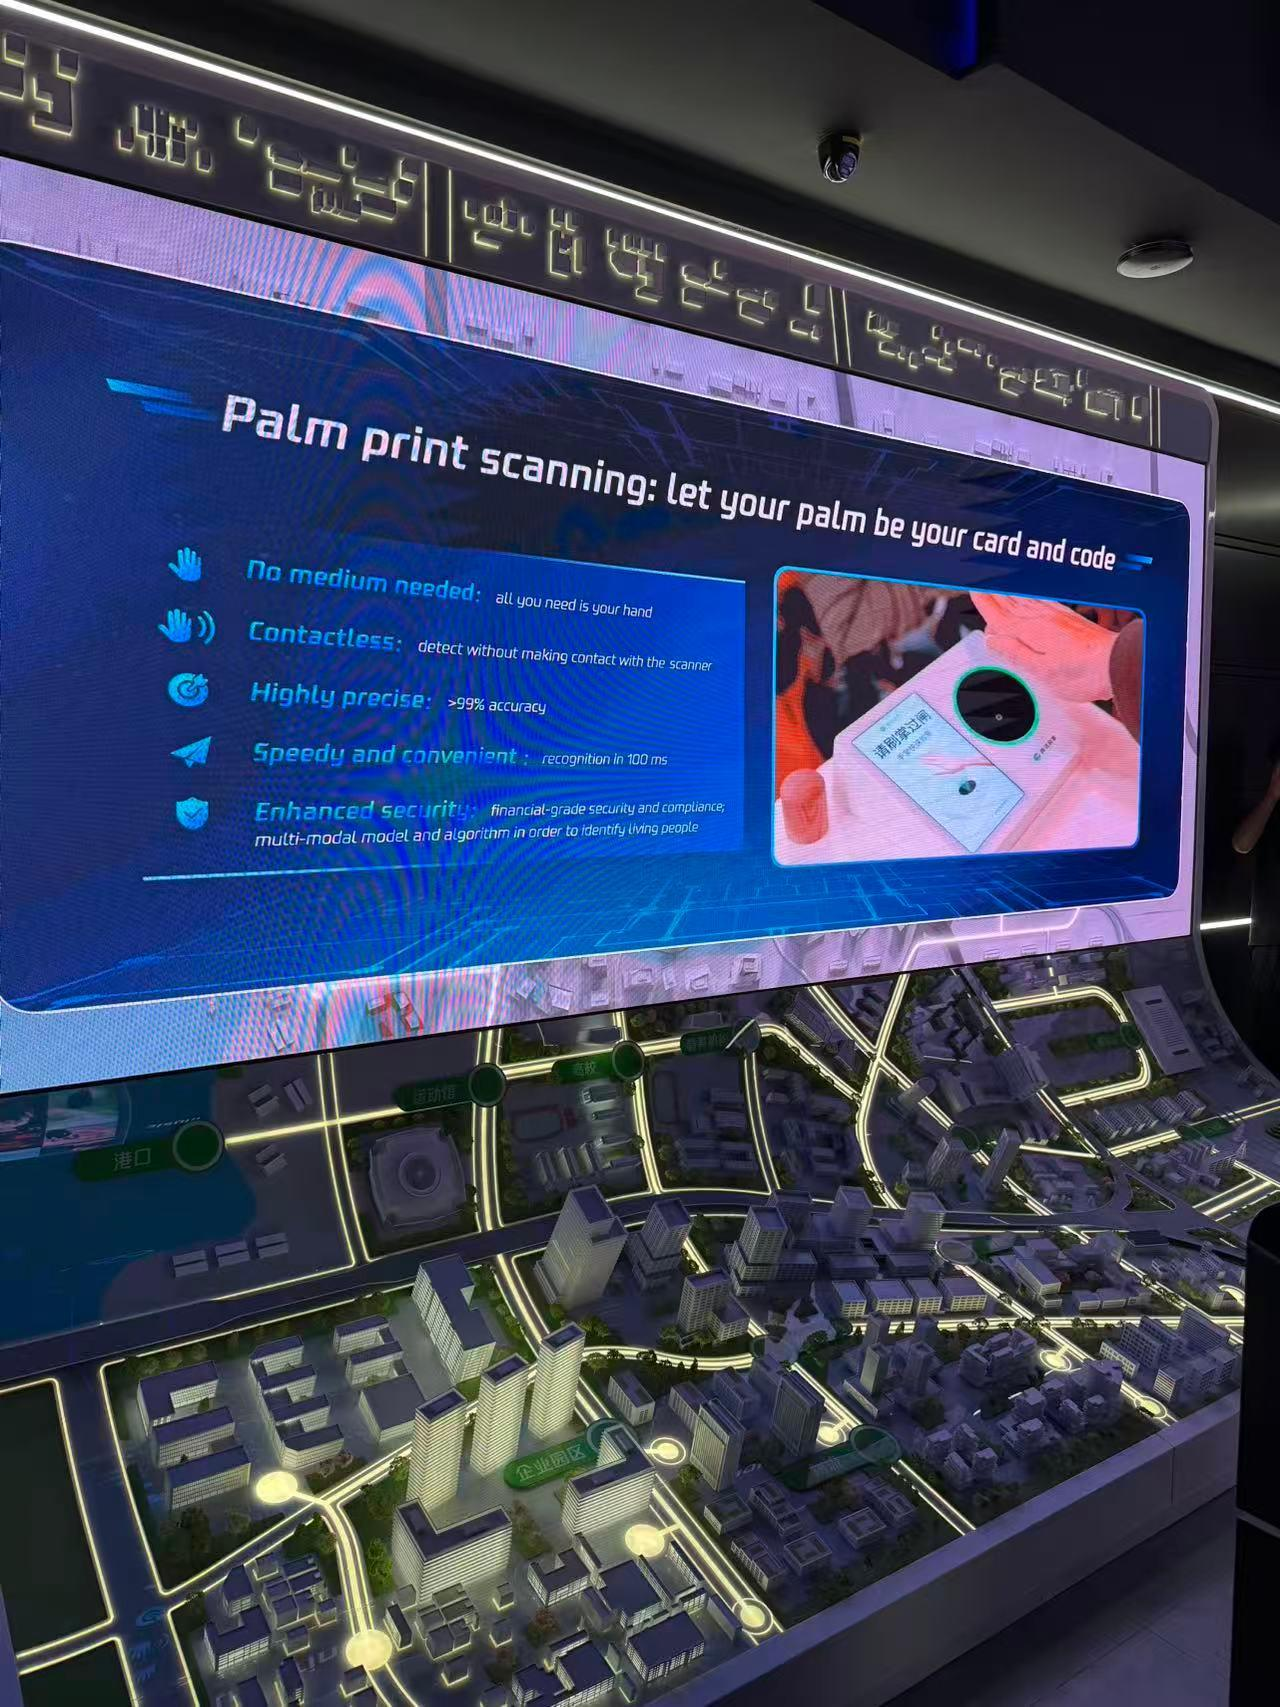
\includegraphics[width=.94\columnwidth,height=4.4cm,keepaspectratio]{figures/field_0.jpg}
\caption{Tencent Shanghai Office, September 4, 2026 field trip. Palm-print identification/payment exhibit. Source: Qianshuo Wang's Intellectual Statement II, Figure 1; photograph by Qianshuo (Aaron) Wang. The display motivates a distinction between technical performance and willingness to rely on technology.}
\Description{Photograph retained from the author's earlier statement showing a Tencent palm-print recognition exhibit for identification and payment.}
\end{figure}
\textbf{Observation versus interpretation.} At the Shanghai Tencent office, I observed a contactless palm-identification / payment display that emphasizes accuracy, speed, and security. \textit{Interpretation:} The display suggested that perceived privacy and security risks may influence willingness to rely on a technology; it does not establish a privacy guarantee or measured adoption effect. MediaPipe~\cite{mediapipe} provided open-source inspiration for on-device perception and privacy-sensitive interaction design, but it does not establish consent, security, or trust. This motivates separating technical capability from reliance and treating privacy as a possible future mechanism rather than a measured PS1 variable.

\begin{figure}[h]
\centering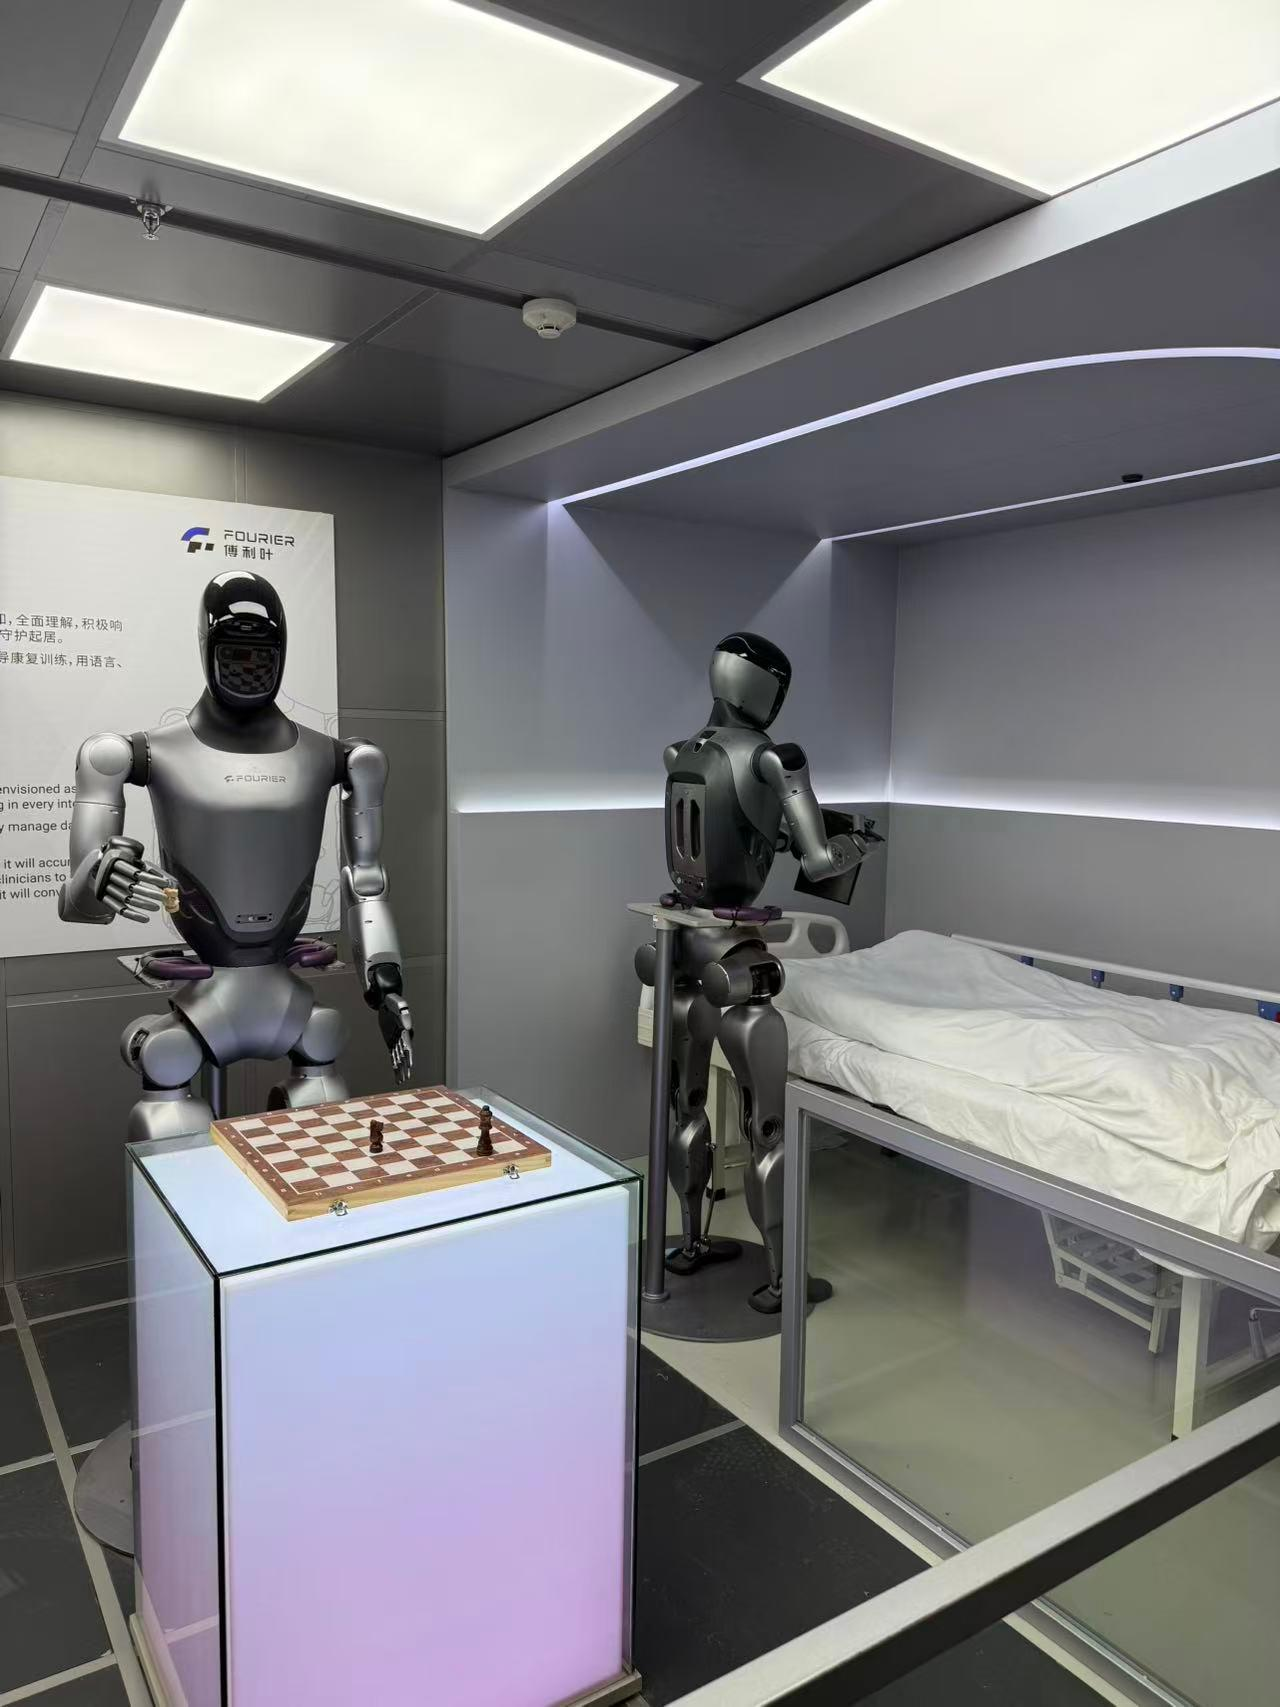
\includegraphics[width=.94\columnwidth,height=4.4cm,keepaspectratio]{figures/field_1.jpg}
\caption{Shanghai Science and Technology Museum, September 4, 2026 field trip. Fourier GRx humanoid robot exhibit. Source: Qianshuo Wang's Intellectual Statement II, Figure 2; photograph by Qianshuo (Aaron) Wang. The exhibit motivates questions about trust in consequential assistance.}
\Description{Photograph retained from the author's earlier statement showing the Fourier GRx humanoid robot beside exhibit information.}
\end{figure}
\textbf{Observation versus interpretation.} At the Shanghai Science and Technology Museum, I observed a humanoid-robot exhibit presenting companionship, workplace assistance, caregiving, and rehabilitation applications. \textit{Interpretation:} The exhibit suggested that willingness to rely on AI or robotic assistance may depend on perceived consequences for well-being, but the observation provides no evidence of clinical effectiveness or user trust. MMPose~\cite{mmpose} provided open-source inspiration for pose analysis, while reinforcing that technical performance alone cannot identify whether a person trusts or relies on assistance. This motivates keeping computational performance, subjective beliefs, and reliance conceptually separate.

\textbf{Value pathway.} The Tencent observation motivates better communication of recommendation uncertainty, while the museum observation motivates consumer education about mistaken reliance. Statement II's SDG 8.2 productivity pathway remains a long-term aspiration; PS1 adds the required SDG 4 learning pathway by combining the game with the expected-payoff benchmark. No productivity or learning improvement has yet been measured.

\section{Review response and revision record} The initial submission is due September 13, 2026; classroom review follows September 14, reviewer follow-up September 16, and revision September 20. At this draft stage, peer reviews, author responses, reviewer follow-up, and v2 are therefore pending. For each completed review, I will record the strength to retain, constructive concern, clarification question, author decision, resulting change, and verification outcome. No reviewer feedback has been fabricated in advance.

\clearpage\onecolumn
\section{Structured abstract and cumulative proposal map}

\begin{table*}[ht]
\caption{Current structured abstract and cumulative proposal map. Prior framing is retained in Intellectual Statement II.}
\label{tab:structured-abstract}
\begin{tabular}{p{0.25\textwidth} p{0.69\textwidth}}
\toprule
\textbf{Proposal element} & \textbf{Current statement / change} \\
\midrule

\textbf{Background}
&
Limited ticket supply makes immediate purchase compete with a possible discount and sell-out. Bounded rationality motivates examining how consumers use AI advice under uncertainty; appropriate reliance requires a defined economic benchmark.
\\

\textbf{Motivation and application}
&
AI advice appears alongside scarcity cues in platform-mediated purchasing scenarios. Consumers, platforms, and educators need to distinguish useful AI advice from decisions that merely appear correct after the outcome.
\\

\textbf{Three connected questions}
&
Economics: when does following AI advice increase expected consumer surplus as competition for scarce tickets changes? Computation: can an inspectable simulator distinguish advice-following from posterior-optimal choice and quantify regret? Behavior: does reliance reflect trust in AI advice or beliefs about sell-out risk? Integrated question: when is AI reliance economically justified given competition, advice reliability, and human beliefs?
\\

\textbf{Method and model assumptions}
&
One focal consumer chooses Buy or Wait after observing market inputs and a noisy recommendation. Other buyers affect an exogenous scarcity probability. Assume $V>P>0$, risk neutrality, a 10\% waiting discount, and a known symmetric signal. The computational benchmark compares always-follow, ignore-advice, and Bayesian posterior-optimal policies across 25 synthetic conditions.
\\

\textbf{Results or expected results}
&
Executed synthetic results: in the default case, always-follow yields expected payoff 66.1657 versus 70 for the posterior-optimal policy (regret 3.8343); a seeded 100,000-round simulation gives 66.202. These are computational results, not human evidence. Human reliance patterns and educational gains remain untested; belief-based explanations could challenge the proposed trust mechanism.
\\

\textbf{Intellectual merits}
&
The proposed contribution connects market incentives, inspectable computation, and behavioral explanations of AI reliance. It separates ex-ante decision quality from ex-post correctness and distinguishes beliefs about market risk from beliefs about AI quality. It does not yet establish an empirical behavioral mechanism or a novel general theorem.
\\

\textbf{Practical impacts}
&
Potential platform value lies in communicating recommendation uncertainty together with its economic consequences. Public value comes from an open-access SDG~4 learning tool that combines predictions, game outcomes, and expected-payoff benchmarks. Learning gains, financial-market transfer, and productivity effects require separate validation.
\\

\textbf{Feedback received and revision made}
&
Session D introduced bounded rationality, trust and reputation, and strategic competition as complementary perspectives. My September 9 Human-Only reflection recorded the key revision: separate AI reliability from market risk and connect economics, computation, and behavioral science. I therefore revised the project from simple advice-following toward a Bayesian economic benchmark plus a proposed behavioral test distinguishing trust from sell-out beliefs. I subsequently reran and independently verified the final computational notebook in Google Colab.
\\

\bottomrule
\end{tabular}
\end{table*}
\end{document}
